\documentclass[aspectratio=169,11pt]{beamer}
\usepackage{booktabs}
\usepackage{amssymb}
\usepackage{tikz}
\usetikzlibrary{arrows.meta,positioning}

\definecolor{ink}{HTML}{1F2933}
\definecolor{accent}{HTML}{1565C0}
\definecolor{soft}{HTML}{E8F0FB}
\definecolor{muted}{HTML}{6B7785}
\definecolor{good}{HTML}{2E7D32}
\definecolor{bad}{HTML}{C62828}
\setbeamercolor{background canvas}{bg=white}
\setbeamercolor{normal text}{fg=ink}
\setbeamercolor{frametitle}{fg=accent}
\setbeamercolor{itemize item}{fg=accent}
\setbeamercolor{itemize subitem}{fg=muted}
\setbeamertemplate{navigation symbols}{}
\setbeamertemplate{itemize item}{\small$\bullet$}
\setbeamertemplate{frametitle}{\vspace{6pt}\textbf{\insertframetitle}\par\vspace{-2pt}{\color{accent}\rule{\textwidth}{0.6pt}}}
\setbeamertemplate{footline}{\hfill{\color{muted}\scriptsize TEAM-89 \quad \insertframenumber\ /\ \inserttotalframenumber}\hspace{10pt}\vspace{6pt}}
\setbeamerfont{frametitle}{size=\Large}

\newcommand{\stat}[2]{\begin{minipage}[t]{0.22\textwidth}\centering{\color{accent}\fontsize{24}{26}\selectfont\textbf{#1}}\\[2pt]{\small #2}\end{minipage}}

\begin{document}

\begin{frame}[plain]
\vspace{30pt}
{\color{accent}\fontsize{30}{34}\selectfont\textbf{CommonsLens}}\\[8pt]
{\Large Automatic category suggestions for Wikimedia Commons}\\[22pt]
{\color{muted}TEAM-89 \quad$\cdot$\quad Problem Statement 3 \quad$\cdot$\quad Final presentation}\\[30pt]
\small Suggest the right categories for a new upload, show the evidence, and say honestly when unsure.
\end{frame}

\begin{frame}{Why this is hard}
\begin{columns}[T]
\column{0.55\textwidth}
\begin{itemize}\setlength{\itemsep}{6pt}
\item \textbf{Huge, growing label space:} 24,486 categories in our sample alone; new ones every day
\item \textbf{Long tail:} 72\% of test labels belong to categories with \emph{no} training image
\item \textbf{Incomplete labels:} a missing category is not a wrong one
\item \textbf{Editors need trust:} why a category is suggested, and when the system does not know
\end{itemize}
\column{0.42\textwidth}
\begin{block}{}
\small A fixed classifier with a softmax head fails all four: it needs retraining for every new
category, ignores the tail, punishes unlabelled parents, and always answers.\\[6pt]
\textbf{Our answer:} categories are \emph{retrievable objects} in a shared image--text space.
\end{block}
\end{columns}
\end{frame}

\begin{frame}{Architecture}
\centering
\resizebox{\linewidth}{!}{%
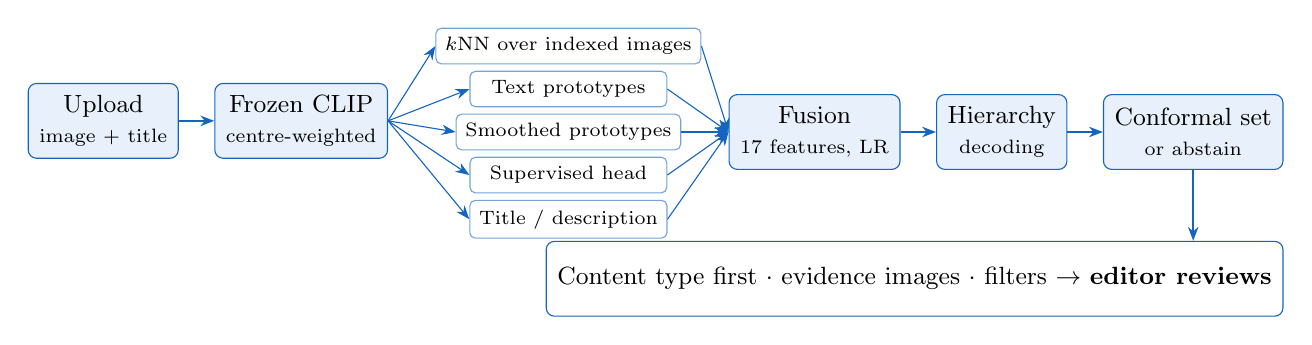
\begin{tikzpicture}[
  box/.style={draw=accent, fill=soft, rounded corners=3pt, align=center, font=\small, minimum height=0.95cm, inner sep=4pt},
  sc/.style={draw=accent!60, fill=white, rounded corners=2pt, font=\scriptsize, minimum width=2.5cm, minimum height=0.45cm},
  ar/.style={-{Stealth[length=5pt]}, thick, accent}]
\node[box] (up) {Upload\\\scriptsize image + title};
\node[box, right=0.45cm of up] (enc) {Frozen CLIP\\\scriptsize centre-weighted};
\node[sc, right=0.6cm of enc, yshift=0.95cm] (s1) {$k$NN over indexed images};
\node[sc, below=0.08cm of s1] (s2) {Text prototypes};
\node[sc, below=0.08cm of s2] (s3) {Smoothed prototypes};
\node[sc, below=0.08cm of s3] (s4) {Supervised head};
\node[sc, below=0.08cm of s4] (s5) {Title / description};
\node[box, right=0.6cm of s3] (fus) {Fusion\\\scriptsize 17 features, LR};
\node[box, right=0.45cm of fus] (hier) {Hierarchy\\\scriptsize decoding};
\node[box, right=0.45cm of hier] (conf) {Conformal set\\\scriptsize or abstain};
\draw[ar] (up) -- (enc);
\foreach \s in {s1,s2,s3,s4,s5} {\draw[ar, thin] (enc.east) -- (\s.west); \draw[ar, thin] (\s.east) -- (fus.west);}
\draw[ar] (fus) -- (hier); \draw[ar] (hier) -- (conf);
\node[box, below=0.9cm of conf.south east, anchor=north east, minimum width=7.2cm, fill=white] (out) {Content type first $\cdot$ evidence images $\cdot$ filters $\rightarrow$ \textbf{editor reviews}};
\draw[ar] (conf.south) -- (conf.south |- out.north);
\end{tikzpicture}}
\vspace{10pt}
\raggedright\small New categories are suggestible instantly; new images and editor accept/reject update the index
without retraining. Fusion runs only on the union of each scorer's top 100 candidates, never on all categories.
\end{frame}

\begin{frame}{What the editor sees}
\begin{columns}[T]
\column{0.5\textwidth}
\begin{itemize}\setlength{\itemsep}{5pt}
\item {\color{accent}$\star$} \textbf{Content type first:} Object, Living thing, Scene, Event or Abstract concept (or two, e.g.\ a fruit market)
\item \textbf{Unsure banner} when the type is below 50\%
\item {\color{good}\checkmark} \textbf{Suggestion set:} the marked rows contain a correct category with a stated probability; empty set $\Rightarrow$ ``manual categorisation''
\item \textbf{Why:} the indexed images and signals behind each suggestion
\end{itemize}
\column{0.47\textwidth}
\begin{itemize}\setlength{\itemsep}{5pt}
\item \textbf{Filters:} no maintenance or contest categories; bare country names and over-specific ones (dates, people counts, non-Latin script) hidden unless very sure
\item \textbf{Report a problem:} testers' reports are stored, de-duplicated and triaged; many fixes came from them
\item \textbf{Public read-only demo} link for anyone
\end{itemize}
\end{columns}
\end{frame}

\begin{frame}{Data and honest evaluation}
\begin{itemize}\setlength{\itemsep}{6pt}
\item \textbf{6,303 Commons files}: 107 topical seeds, 48 region seeds (8 countries per continent), 1,500 uniformly random files
\item \textbf{Temporal split} by upload time (4,429 / 937 / 937), perceptual-hash and embedding de-duplication
\item \textbf{Realistic validation:} vocabulary built from training data only, so tuning sees unknown categories like the test set does \\
{\small\color{muted} this fixed a validation--test gap of .135 $\rightarrow$ .014}
\item \textbf{Bias audit} per topic and per region; robustness to blur, JPEG and downscaling; latency and memory
\item \textbf{77 automated tests}, plus two hand-labelled test packs for the content type
\end{itemize}
\end{frame}

\begin{frame}{Results on 937 unseen, later uploads}
\vspace{4pt}
\stat{.348}{P@1 with a title}\hfill\stat{.336}{R@10 with a title}\hfill\stat{+53\%}{fusion vs best single scorer}\hfill\stat{30\,ms}{per image on a laptop}
\vspace{14pt}
\begin{columns}[T]
\column{0.48\textwidth}
\small
\begin{tabular}{@{}lrr@{}}
\toprule
F1@5 & +meta & image only \\ \midrule
Full fusion & \textbf{.152} & \textbf{.085} \\
Lexical (title words) only & .099 & -- \\
Smoothed prototypes only & .083 & -- \\
$k$NN only & .069 & -- \\ \bottomrule
\end{tabular}
\column{0.48\textwidth}
\small
\begin{tabular}{@{}lrr@{}}
\toprule
Recall@5 by category size & labels & R \\ \midrule
20+ images & 380 & .821 \\
5--19 & 217 & .439 \\
1--4 & 318 & .200 \\
unseen & 2,412 & .003 \\ \bottomrule
\end{tabular}
\end{columns}
\vspace{8pt}
\small The tail is the bottleneck: only 36\% of test labels are in the vocabulary at all.
\end{frame}

\begin{frame}{What worked, what did not}
\begin{columns}[T]
\column{0.49\textwidth}
\textbf{Smoothed prototypes} {\small(M1's core idea)}
\begin{itemize}\small\setlength{\itemsep}{3pt}
\item {\color{good}Image centroids}: prototype recall$\times$10 (.020 $\rightarrow$ .191)
\item {\color{muted}Full system unchanged} (.152): $k$NN already carries it
\item {\color{bad}Parent/sibling term hurt the tail} (.061 $\rightarrow$ .030), so it was not used
\item {\color{bad}Replacing text prototypes} broke title matching; kept as a separate signal
\end{itemize}
\column{0.49\textwidth}
\textbf{Conformal suggestion sets}
\begin{itemize}\small\setlength{\itemsep}{3pt}
\item Sets adapt: at $\alpha{=}0.4$ median 3 categories, beats a fixed top-3 (.518 vs .484)
\item 7\% of uploads routed to manual categorisation
\item {\color{bad}Coverage 7--8 points under target}: later uploads break exchangeability $\Rightarrow$ recalibrate on recent uploads
\end{itemize}
\end{columns}
\vspace{10pt}
\small\color{muted} We also caught two evaluation pitfalls: a leaky validation vocabulary, and a display filter inside the ranker that scored every region at zero.
\end{frame}

\begin{frame}{Fairness, robustness, responsibility}
\begin{columns}[T]
\column{0.42\textwidth}
\small
\begin{tabular}{@{}lrrr@{}}
\toprule
F1@5 & $n$ & +meta & image \\ \midrule
Europe & 42 & .274 & .037 \\
Africa & 71 & .207 & .006 \\
S.\ America & 48 & .087 & .009 \\
Asia & 47 & .087 & .034 \\
N.\ America & 43 & .036 & .012 \\ \bottomrule
\end{tabular}\\[6pt]
\scriptsize\color{muted} Small groups: gaps are indicative.
\column{0.55\textwidth}
\begin{itemize}\small\setlength{\itemsep}{4pt}
\item \textbf{Titles matter for places}: image-only accuracy is near zero in every region
\item \textbf{Robust}: heavy blur costs 5\% with a title, 36\% without
\item \textbf{Licences}: trained only on openly licensed Commons files; ObjectNet, WIDER FACE, DTD and COCO were \emph{not} used (training or commercial restrictions)
\item \textbf{People}: typed as living things, never identified
\item \textbf{Human in the loop}: nothing is applied automatically
\end{itemize}
\end{columns}
\end{frame}

\begin{frame}{Content type and the feedback loop}
\begin{columns}[T]
\column{0.48\textwidth}
\textbf{Trained content-type classifier}
\begin{itemize}\small\setlength{\itemsep}{3pt}
\item 939 openly licensed photos, equal share per source category
\item 82.9\% on held-out photos, five types
\item Living-things pack (250): 91.6\% typed Living thing; 88.6\% on the 88 hard photos
\item Portraits (4 of 14) traced to a collection bug: fixed
\end{itemize}
\column{0.48\textwidth}
\textbf{Fixed from tester reports}
\begin{itemize}\small\setlength{\itemsep}{3pt}
\item People pulled to ``Marathons'' $\rightarrow$ centre-weighted embedding
\item Cathedral typed Object $\rightarrow$ buildings are Scenes
\item Mushroom, portrait $\rightarrow$ Living thing type
\item ``3 men 1 woman'', dates, Urdu text $\rightarrow$ hidden unless sure
\item ``Wiki Loves \dots'' contest categories $\rightarrow$ filtered
\end{itemize}
\end{columns}
\end{frame}

\begin{frame}{Scale and next steps}
\begin{columns}[T]
\column{0.48\textwidth}
\textbf{Built to grow}
\begin{itemize}\small\setlength{\itemsep}{3pt}
\item Frozen encoder: no GPU training; scoring 1\,ms per image
\item FAISS flat, HNSW or IVF-PQ index by configuration
\item New categories and images live without retraining
\item MIT licence; runs on a laptop
\end{itemize}
\column{0.48\textwidth}
\textbf{Next}
\begin{itemize}\small\setlength{\itemsep}{3pt}
\item Grow the vocabulary and the tail: multilingual names, geotags
\item Rolling conformal recalibration on recent uploads
\item SigLIP vs CLIP; newest-uploads test set (tools built)
\item Human-reviewed score: many ``wrong'' suggestions are valid
\end{itemize}
\end{columns}
\vspace{16pt}
\centering\large\color{accent}\textbf{CommonsLens: suggestions editors can check, and honesty when unsure.}
\end{frame}

\end{document}
